\documentclass{article}

% if you need to pass options to natbib, use, e.g.:
% \PassOptionsToPackage{numbers, compress}{natbib}
% before loading nips_2018

% ready for submission
%\usepackage{nips_2018}

% to compile a preprint version, e.g., for submission to arXiv, add
% add the [preprint] option:
\usepackage[final]{nips_2018}

% to compile a camera-ready version, add the [final] option, e.g.:
% \usepackage[final]{nips_2018}

% to avoid loading the natbib package, add option nonatbib:
% \usepackage[nonatbib]{nips_2018}

\usepackage[utf8]{inputenc} % allow utf-8 input
\usepackage[T1]{fontenc}    % use 8-bit T1 fonts
\usepackage{hyperref}       % hyperlinks
\usepackage{url}            % simple URL typesetting
\usepackage{booktabs}       % professional-quality tables
\usepackage{amsfonts}       % blackboard math symbols
\usepackage{nicefrac}       % compact symbols for 1/2, etc.
\usepackage{microtype}      % microtypography
\usepackage{graphicx}       % include graphics

\title{Analysis of Generating Isolated Tracks from NES Music}

% The \author macro works with any number of authors. There are two
% commands used to separate the names and addresses of multiple
% authors: \And and \AND.
%
% Using \And between authors leaves it to LaTeX to determine where to
% break the lines. Using \AND forces a line break at that point. So,
% if LaTeX puts 3 of 4 authors names on the first line, and the last
% on the second line, try using \AND instead of \And before the third
% author name.

\author{
  Bryan Learn\\
  blearn@andrew.cmu.edu\\
  Carnegie Mellon University\\
  Pittsburgh, PA 15213\\
  \And
  Mike Tasota\\
  tasota@andrew.cmu.edu\\
  Carnegie Mellon University\\
  Pittsburgh, PA 15213\\
}

\begin{document}
% \nipsfinalcopy is no longer used

\maketitle


\begin{abstract}
By using a dataset based on the Nintendo audio synthesizer with well-defined noise and wave generators, we were able to automate the process of training models on isolated tracks to learn note structure without conditioning on specific MIDI channels or instruments. Models from the Magenta project were used for training and generating music. With a dataset of approximately five thousand songs, our results indicated that the recurrent neural network model was more successful than the variational autoencoder model in generating note sequences on the isolated tracks. Our work has also suggested reasons for preferring the MelodyRNN model over the DrumsRNN model when learning isolated percussive tracks.
\end{abstract}


\section{Introduction}


Although similar to text generation in many respects, there is still significant progress to be made in the area of music generation. There are a few distinctions between the problem of music generation and text generation that affect this. The number of potential states that a standard 88-key piano can take greatly exceeds the number of words in any language. 
Multiple voices and tempo also increases the complexity of music generation.

But music is much more than just playing a combination of frequencies over an interval of time. There are several types of voices and classes of instruments that music can take on, from percussion and bass to chords and melodies. And although several attempts already exist to learn instrument classes (Song from PI [1], MuseGAN [4]), these implementations work on fixed sets of instruments and introduce chord conditioning to keep the generated harmony fixed. In this paper we explore using deep learning models to learn isolated tracks from a dataset. We also explore the potential for removing instrument and chord restrictions to see how much can be learned by the models alone.


\section{Related Work}


In the MidiNet paper, Yang et al. created a CNN-GAN based model for MIDI generation [4]. They propose that their model could be possibly expanded to generate multiple tracks. This was demonstrated in the work done by MuseGAN. However, MuseGAN works with a fixed set of instruments, namely bass, drums, guitar, piano, and strings. Another related work in multiple track generation is from Chu et al. in their "Song from PI" RNN. Although it is capable of producing multiple tracks, it also conditioned the generation on scale types to help pick up regularities in their dataset [1].

\subsection{Magenta}

In our work, we explored learning isolated tracks by using the deep learning models in the Magenta project. Magenta is a research project from the Google Brain team that explores the role of machine learning in creating art and music. Utilizing the TensorFlow library, Magenta publishes its deep learning models for other researchers to use. For our work, we focused on two of the learning models. MelodyRNN implements melody generation using long short-term memory (LSTM) cells inside of a recurrent neural network. MusicVAE is a hierarchical recurrent variational autoencoder which learns a latent space of musical sequences.


\section{Dataset}

The suggested input data for the music generation project topic was classical piano music pieces from the website (www.piano-midi.de). We ultimately decided against this dataset because of its lack of well-defined tracks and sparse variety of instrument voices across all MIDI files. On top of this, the classical piano dataset was relatively small (less than 1,000 MIDI files). For our work, it was necessary to have access to a dataset of MIDI files which had consistent track types across the entire dataset. To accomplish this, we used the NES Music Database (NES-MDB) as presented by Donahue et al. [2]. The dataset consists of 5,278 songs from the soundtracks of 397 NES games. Each MIDI file consists of four instrument voices, each mapping to an NES synthesizer. These voices are two pulse-wave generators (P1, P2), a triangle-wave generator (TR), and a percussive noise generator (NO). Since these voices are consistent throughout all files in the dataset, we assumed that each voice represented a specific track type. For example, the percussive noise generator would be a drum track for all MIDI files in which it is defined.


\section{Methods}

To train on specific voices, we modified the original MIDI dataset to generate four single-track datasets for each of the four tracks present (P1, P2, TR, NO). This was achieved using the midicsv and csvmidi tools developed by John Walker. By converting MIDI files to CSV format, we were able to automate the process of extracting isolated tracks from each file in the dataset. Then we passed each of the modified single-track datasets through the MelodyRNN and MusicVAE pipeline. After training was initialized, the Magenta models generated event files which include the training loss from the model at specific checkpoints.

It is also worth noting that the dataset with the isolated drums track (NO) had to be modified further to properly train on the MelodyRNN model. As per the General MIDI standard, channel 10 is dedicated to percussion, and the first step taken by MelodyRNN was to remove all notes on this channel. To resolve this, we simply modified our script for the isolated drums track to also modify the track’s MIDI channel.



\section{Experiments}

Since our interests lie in learning individual voice classes, we used models trained on the original dataset as well as models trained on the four individual voice classes (P1, P2, TR, and NO). This allowed us to audibly compare differences in what the baseline model learned to what our voice-specific models learned. Also, for RNN, we compared our isolated track models to the baseline model from their calculated training losses.

\subsection{Training the Baseline}
We wanted a baseline comparison for the two Magenta models that we considered (MusicVAE and MelodyRNN). To accomplish this, we trained with the original NES-MDB Dataset with all four voices. For the MusicVAE baseline we used the Trio configuration, where "trio" refers to an ensemble of three performers or voices. MusicVAE’s trio consists of melody, bass, and drums, and it uses chord conditioning to keep harmony fixed. We also trained the MelodyRNN baseline model, but the MelodyRNN configuration only produces one melody in contrast to the trio.

\subsection{Isolated Track Training}
We trained both the MusicVAE model and the MelodyRNN model on each of the four isolated tracks to create a total of 8 track-separated models. Each model was trained up to 8 hours. We noticed the MelodyRNN models that were trained for 8 hours were overfitting. To address this, we compared the performance of earlier versions of the models to the overfit models by evaluating test loss.

When training drums for MelodyRNN, we learned that the basic MelodyRNN configuration ignored all information from the MIDI channel associated with percussion. For learning drums, a separate model exists in the Magenta project (DrumsRNN). However, our training indicated that training percussion on DrumsRNN only produces one note value despite having multiple percussive note values in the training data. We successfully preserved this information in the training by modifying the MIDI files in our NO dataset to use a non-percussive MIDI channel and training with MelodyRNN. This can also be seen in Figure 4, where "no" indicates DrumsRNN and "no2" indicates MelodyRNN.


\begin{figure}[htb!]
  \begin{minipage}{0.48\textwidth}
    \centering
    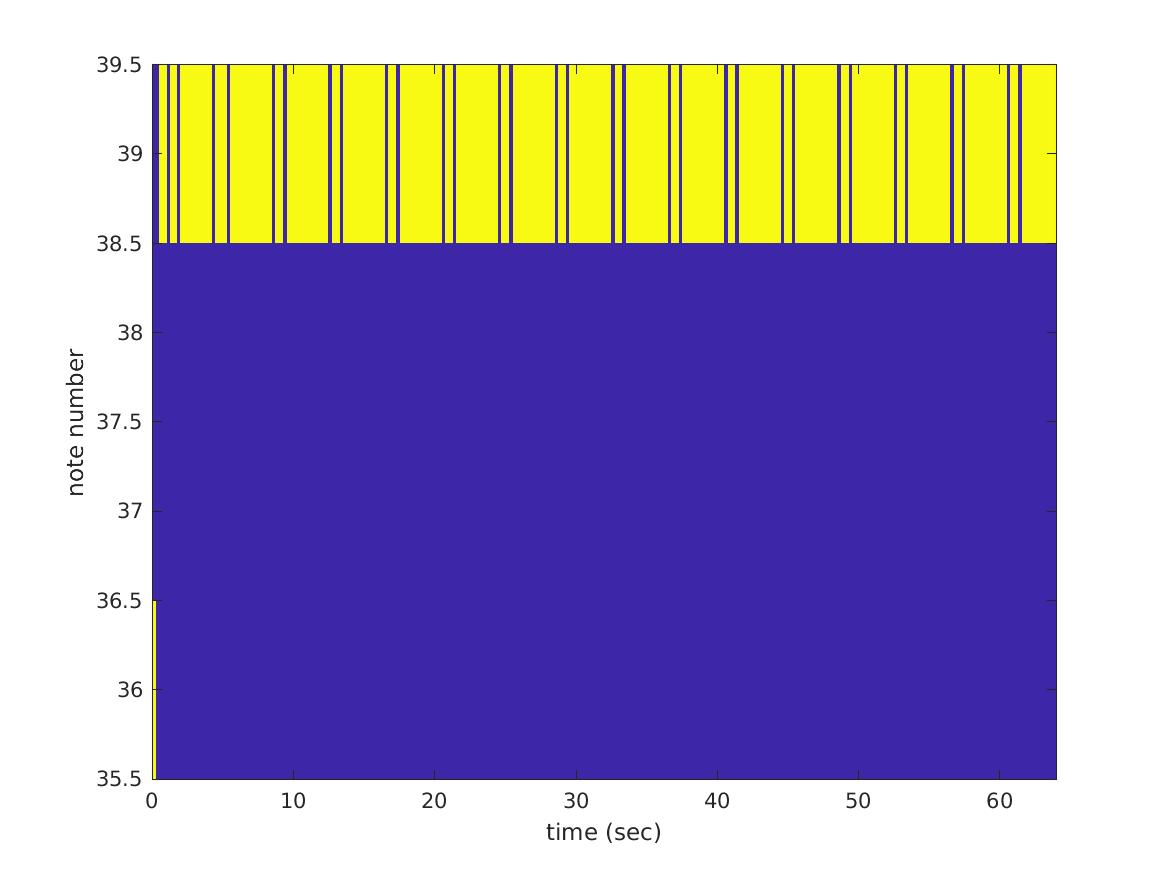
\includegraphics[height=4cm, width=4cm]{img/DrumRNN_drum.jpg}
    \caption{DrumsRNN: percussive track}
  \end{minipage}\hfill
  \begin{minipage}{0.48\textwidth}
    \centering
    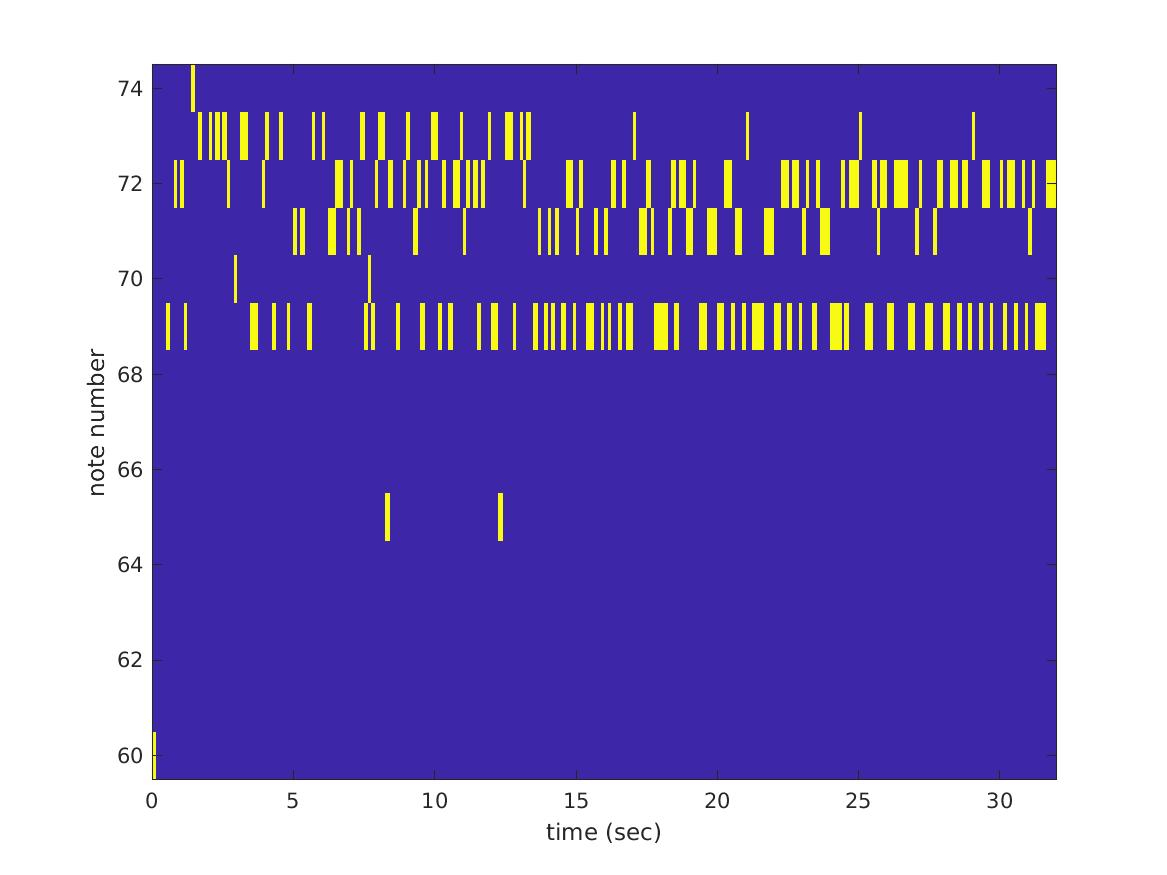
\includegraphics[height=4cm, width=4cm]{img/MelodyRNN_drum.jpg}
    \caption{MelodyRNN: percussive track}
  \end{minipage}
\end{figure}

\subsection{Generated Tracks}
After generating the isolated tracks, we were interested in converting the generated MIDI files into synthesized NES tracks. As part of the NES-MDB project, there is a tool for converting MIDI files from the dataset into audio files generated from synthesized track voices. However, we learned that the generated format from the models was not enough to generate synthesized voices. This is because the original dataset included MIDI control event information to produce more expressive voices, and this information was not generated as output from the models.

\begin{figure}[htb!]
  \begin{minipage}{1.0\textwidth}
    \centering
    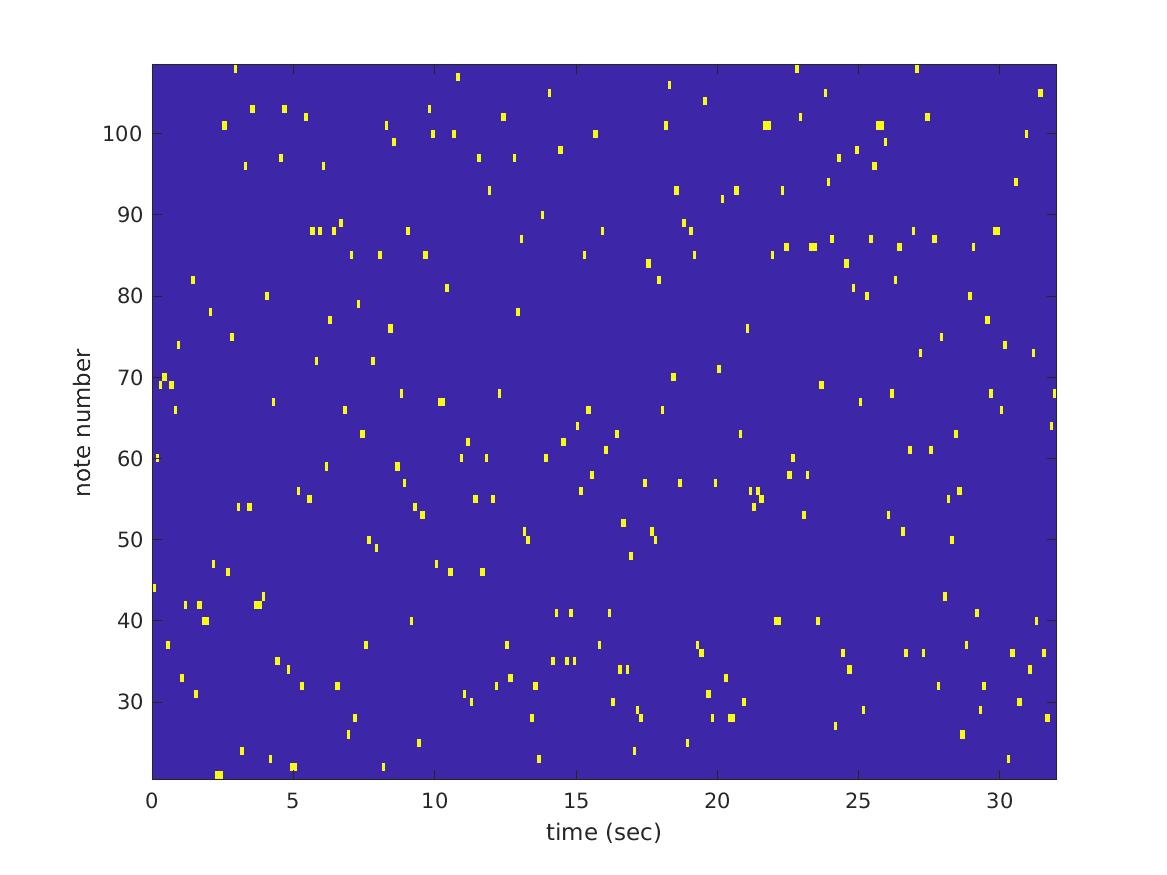
\includegraphics[height=4cm, width=4cm]{img/vae_no.jpg}
    \caption{MusicVAE: percussive track}
  \end{minipage}
\end{figure}

\section{Results}


We evaluated the trained models by listening to the generated music and comparing the training loss across model types. For MelodyRNN, the training loss trend for each isolated track was less than the training loss for the baseline model. The graph for training loss in the MusicVAE model only includes models which trained beyond the initial checkpoint (P1, P2, TR). When considering the number of isolated tracks that were learned, the RNN models outperform the VAE models. The MusicVAE baseline and percussive track (NO) never went beyond the initial checkpoint in training. This resulted in the models generating mostly random noise (see Figure 3). For MusicVAE, it is interesting that training never went beyond the initial checkpoint for all training data that included percussion. Even when modifying the files to use a non-percussive MIDI channel type, the MusicVAE model failed to train beyond its initial checkpoint.

\begin{figure}[htb!]
  \begin{minipage}{0.48\textwidth}
    \centering
    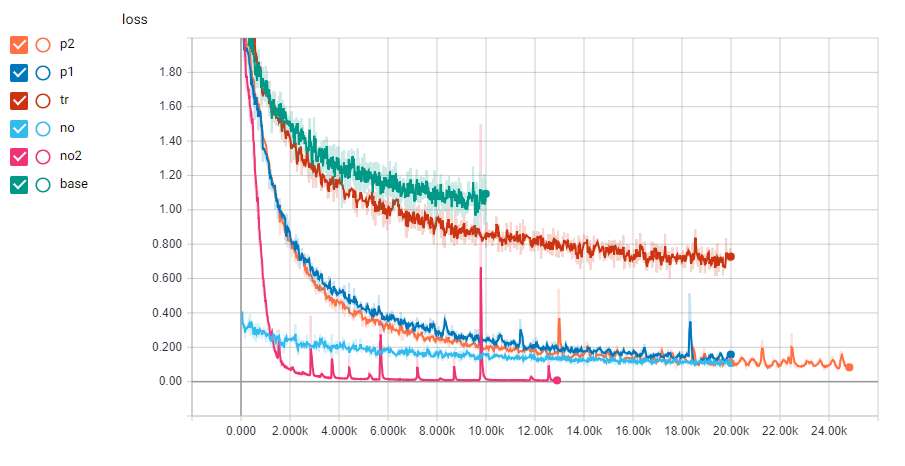
\includegraphics[height=4cm, width=8cm]{img/rnn_loss_all.png}
    \caption{MelodyRNN: training loss}
  \end{minipage}\hfill
  \begin{minipage}{0.48\textwidth}
    \centering
    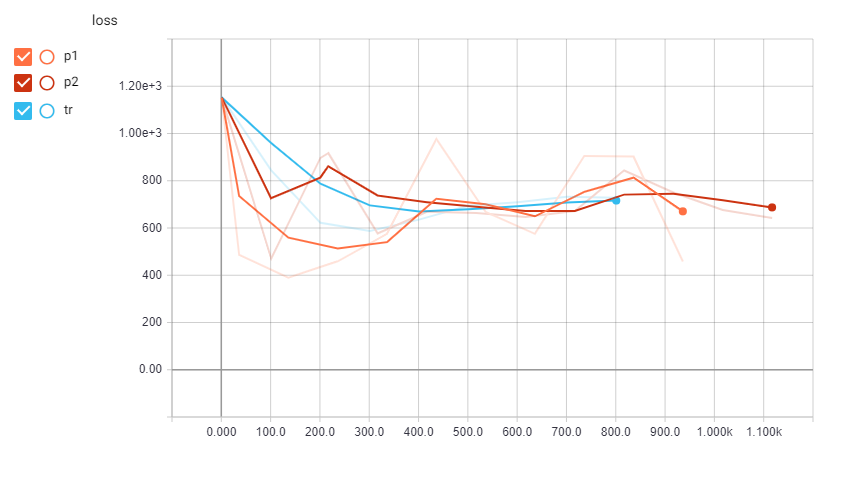
\includegraphics[height=4cm, width=8cm]{img/vae_loss.png}
    \caption{MusicVAE: training loss}
  \end{minipage}
\end{figure}

An additional evaluation on listening to the generated music indicated that the RNN models produced better results than the VAE models (see Figure 6). These results were surprising as our preliminary results seemed to indicate that the MusicVAE model was capable of generating more interesting melodies. This prior analysis was based on pre-trained models provided by the Magenta project. For the MusicVAE model, the training set consisted of over 1.5 million MIDI files scraped over the web [3]. Compared to the size of the NES-MDB dataset, it is likely that the shortcomings of our results for the VAE models were from a lack of training data.


\begin{figure}[htb!]
  \begin{minipage}{1.0\textwidth}
    \centering
    \includegraphics[height=4cm, width=6cm]{img/generated-tracks.png}
    \caption{Top row: MusicVAE; Bottom row: MelodyRNN}
  \end{minipage}
\end{figure}


\section{Conclusion and Future Work}

Our experiments indicate that a recurrent neural network model performed the task of learning isolated tracks from the NES-MDB dataset better than a variational autoencoder model. We would expect this result to hold for any dataset of similar size, but it is still to be determined if similar results would follow in a larger dataset (100,000 or 1 million files) that share the same set of instrument classes. In the future, we would like to see an extension of the MelodyRNN model that is capable of generating MIDI control change events and any other information necessary to render synthesized audio in the NES Music Database format. Extending the model to also generate multiple tracks within a single MIDI file (such as the trio for MusicVAE, minus the chord conditioning) also seems attainable.

\section{Acknowledgements}
This work used the Bridges system, which is supported by NSF award number ACI-1445606, at the Pittsburgh Supercomputing Center (PSC).

We thank our project mentor Jing Mao for guidance, along with Daniel Bird and the rest of the teaching assistants.

For automating the process of isolating the tracks, we use the midicsv and csvmidi programs authored by John Walker. We implore the curious researcher to visit his website (www.fourmilab.ch).

\section*{References}

\small

[1] Chu, Hang, et al. "Song From PI: A Musically Plausible Network for Pop Music Generation." {\it [1611.03477] Song From PI: A Musically Plausible Network for Pop Music Generation,} 10 Nov. 2016, arxiv.org/abs/1611.03477.

[2] Donahue, Chris et al. "The NES Music Database: A multi-instrumental dataset with expressive performance attributes" {\it [1806.04278] The NES Music Database: A multi-instrumental dataset with expressive performance attributes,} 12 June 2018, arxiv.org/abs/1806.04278.

[3] Engel, Jesse, et al. "Latent Constraints: Learning to Generate Conditionally from Unconditional Generative Models." {\it[1711.05772] Latent Constraints: Learning to Generate Conditionally from Unconditional Generative Models.,} 21 Dec 2017, arxiv.org/abs/1711.05772

[4] Yang, Li-Chia, et al. "MidiNet: A Convolutional Generative Adversarial Network for Symbolic-Domain Music Generation." {\it[1703.10847] MidiNet: A Convolutional Generative Adversarial Network for Symbolic-Domain Music Generation,} 18 July 2017, arxiv.org/abs/1703.10847.


\end{document}
